% --------- Initialization ---------- % 
\documentclass[aspectratio=169]{beamer}
\usetheme{default}
\setbeamertemplate{navigation symbols}{}

% Packages
\usepackage{hyperref}
\definecolor{links}{HTML}{2A1B81}
\hypersetup{colorlinks,linkcolor=,urlcolor=links}
\usepackage{graphicx} 

% Personalise Font
\usefonttheme{professionalfonts} % using non standard fonts for beamer
\usefonttheme{serif}% default family is serif
\usepackage{mathpazo}

% Create Transitioning Slides at each section
\AtBeginSection[]{
	\begin{frame}
		\vfill
		\centering
		\begin{beamercolorbox}[sep=8pt,center,shadow=true,rounded=true]{title}
			\usebeamerfont{title}\insertsectionhead\par%
		\end{beamercolorbox}
		\vfill
	\end{frame}
}

% Miniframes Structure
\useoutertheme[subsection=false]{miniframes}
\makeatletter
\let\beamer@writeslidentry@miniframeson=\beamer@writeslidentry
\def\beamer@writeslidentry@miniframesoff{%
	\expandafter\beamer@ifempty\expandafter{\beamer@framestartpage}{}% does not happen normally
	{%else
		% removed \addtocontents commands
		\clearpage\beamer@notesactions%
	}
}
\newcommand*{\miniframeson}{\let\beamer@writeslidentry=\beamer@writeslidentry@miniframeson}
\newcommand*{\miniframesoff}{\let\beamer@writeslidentry=\beamer@writeslidentry@miniframesoff}


\title{Introduction to GitHub}
\author{Fabrizio Leone \\ Python-do-ECARES}

% --------- Document stars here ----------- %
\begin{document}
\begin{frame}[plain]
    \maketitle
\end{frame}

% INTRO
\section{Introduction}

\begin{frame}{Git and GitHub}

\begin{itemize}\setlength\itemsep{2.5em}
	\item Git is a version control system, i.e. a way to keep track of the whole history of things you do on a file. It is useful to save, manage and edit all the different versions of your project. 
	\item GitHub is a web service that allows to conveniently work with Git. It allows you to create your own directories, see projects of other people and collaborate with them. 
	\item You can read more about Git and GitHub \href{https://medium.com/@abhishekj/an-intro-to-git-and-github-1a0e2c7e3a2f}{here} and \href{https://medium.com/launch-school/understanding-git-and-github-8ac987877a5}{here}.
	
\end{itemize}

\end{frame}

\begin{frame}{GitHub Desktop}

\begin{itemize}\setlength\itemsep{2em}
		\item In this course, we interact with GitHub mostly through the GitHub Desktop application.
		\item GitHub Desktop provides a simple yet powerful desktop interface to GitHub.
		\item You can download GitHub desktop \href{https://desktop.github.com/}{here}. 
		\item You can also interact with GitHub using the \href{https://github.com/codepath/ios_guides/wiki/Using-Git-with-Terminal}{Terminal} (not covered in this class).
\end{itemize}	

\end{frame}

% GitHub Desktop
\section{First Steps With GitHub Desktop}

\begin{frame}{Step 1. Clone Repository}{Go to \href{https://github.com/Python-do-ECARES/Classes}{Classes} repository on GitHub and click on the "Clone or download" button.}
\begin{figure}
	\centering
	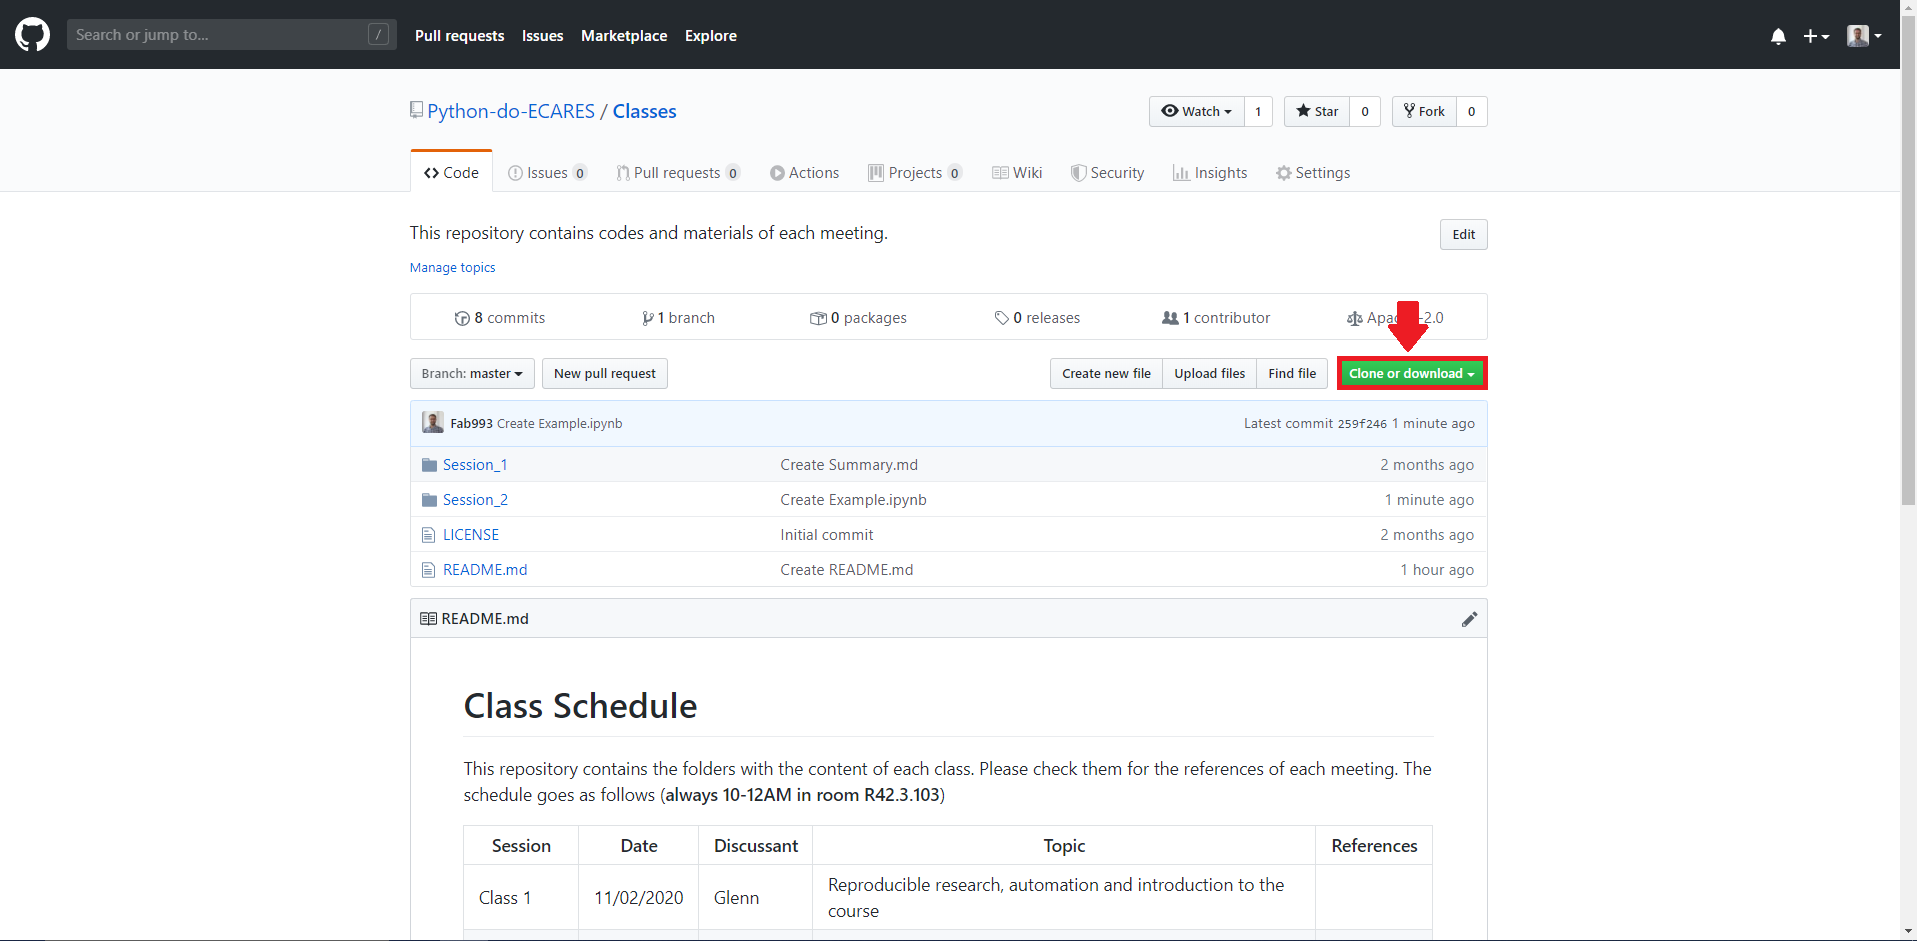
\includegraphics[width=0.9\linewidth]{../images/step1}
\end{figure}
\end{frame}

\begin{frame}{Step 1.A Open Repository}{Choose "Open in Desktop".}	
	\begin{figure}
		\centering
		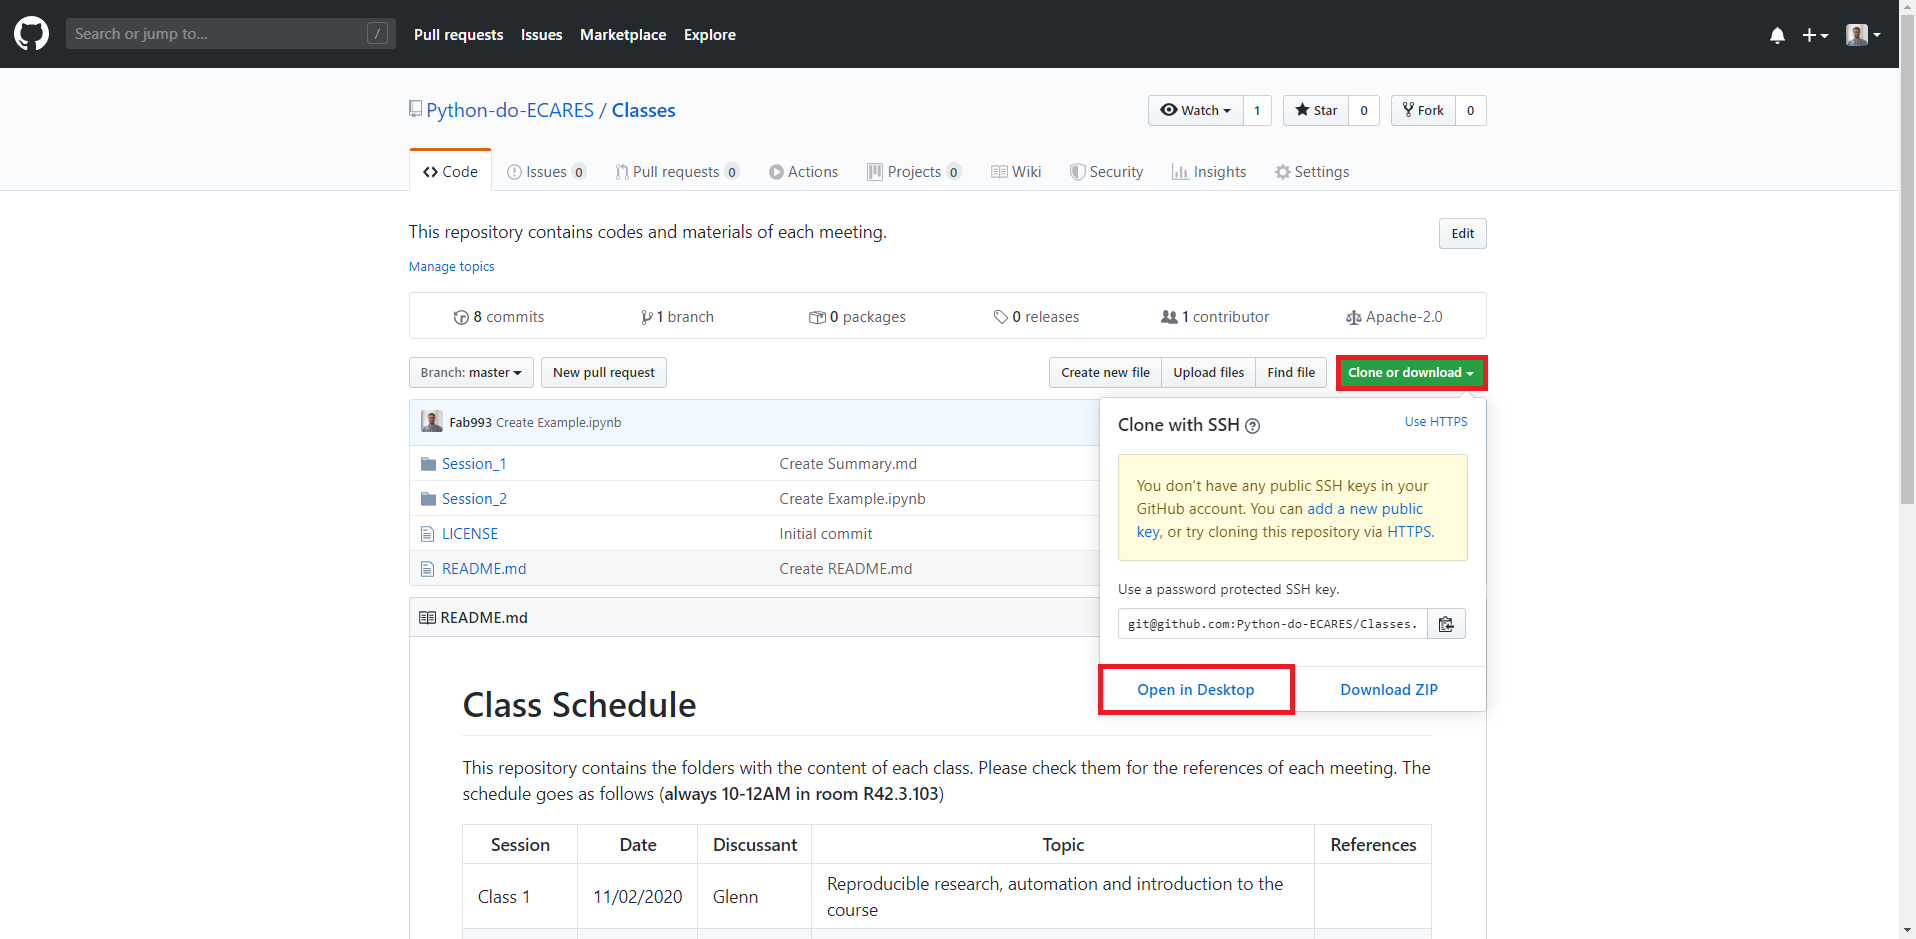
\includegraphics[width=0.9\linewidth]{../images/step1.A}
	\end{figure}
\end{frame}

\begin{frame}{Step 1.B Clone Repository}{Check the local path where to clone the repository and click "Clone".}
	\begin{figure}
		\centering
		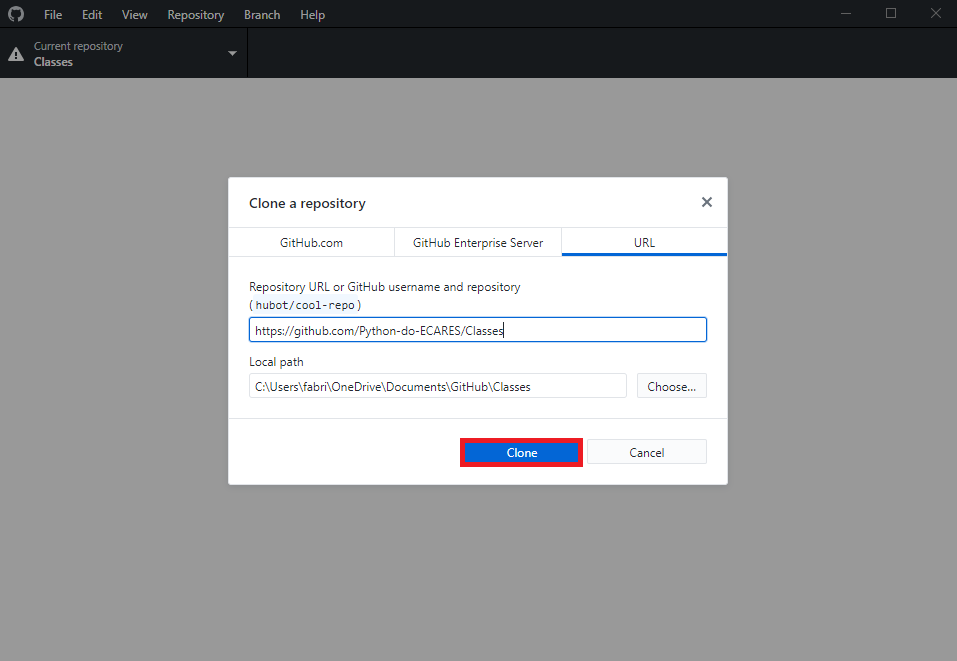
\includegraphics[width=0.7\linewidth]{../images/step1.B}
	\end{figure}
\end{frame}

\begin{frame}{Step 1.C Open Local Directory}{Under GitHub Desktop/Classes/Session$\_2$ you will see the following files.}
	\begin{figure}
		\centering
		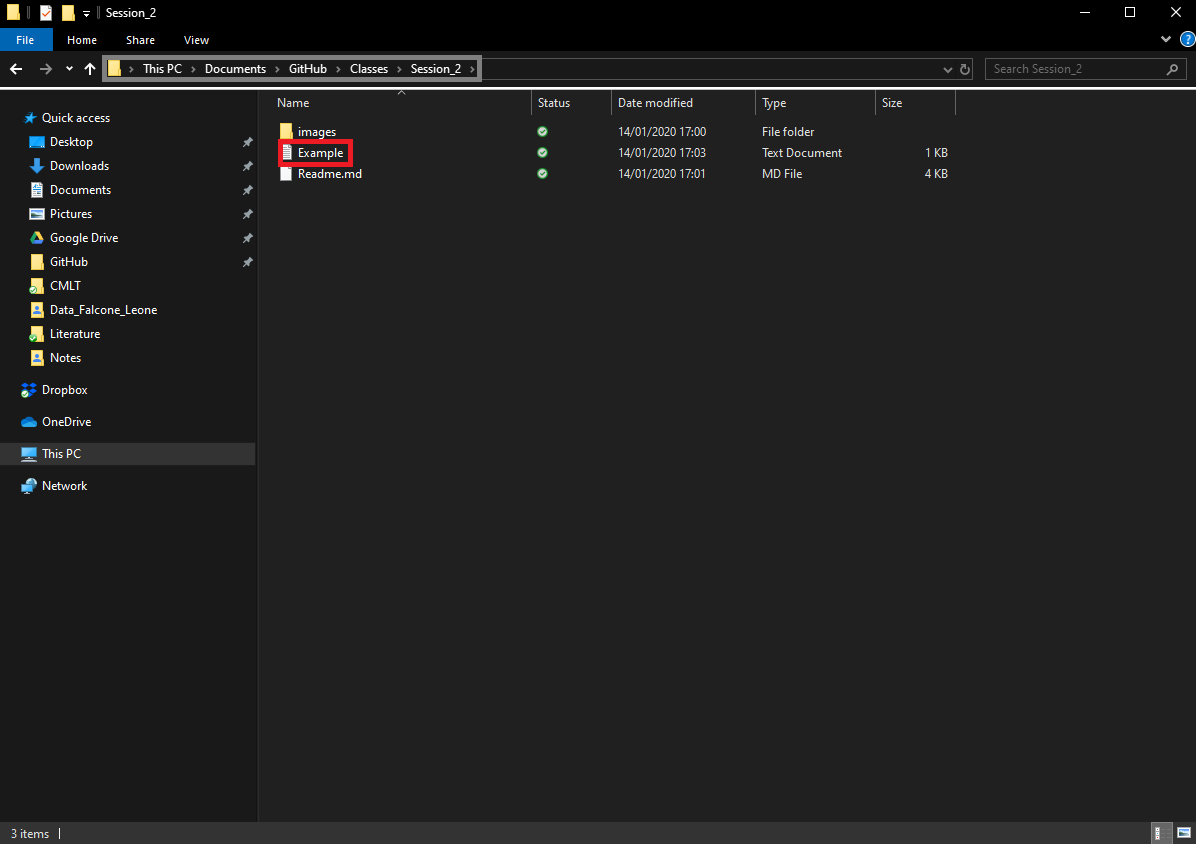
\includegraphics[width=0.7\linewidth]{../images/step1.C}
	\end{figure}
\end{frame}

\begin{frame}{Step 2 Make Changes}{Open \emph{Example.txt}. Add a comment line with your name.}
	\begin{figure}
		\centering
		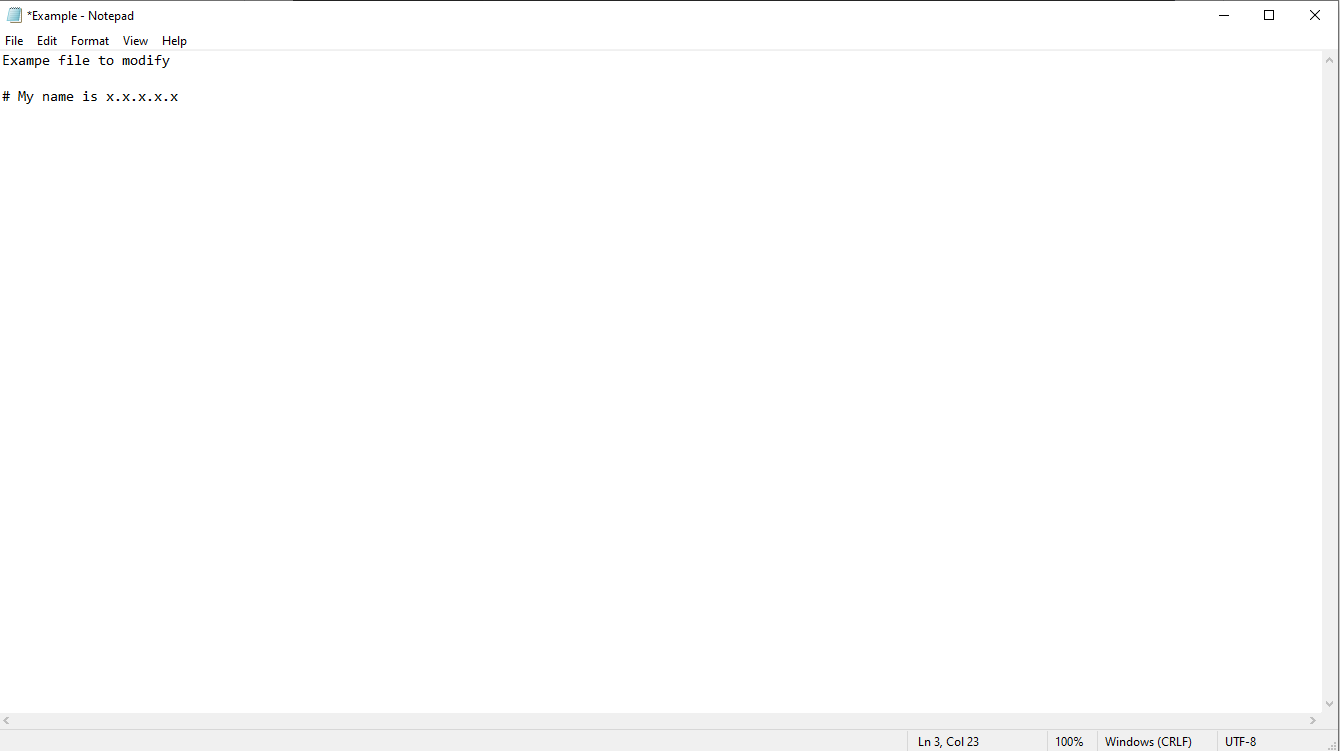
\includegraphics[width=0.8\linewidth]{../images/step2}
	\end{figure}
\end{frame}

\begin{frame}{Step 2.A Save Changes}{Save the file. Changes will be displayed in GitHub Desktop as follows.}
	\begin{figure}
		\centering
		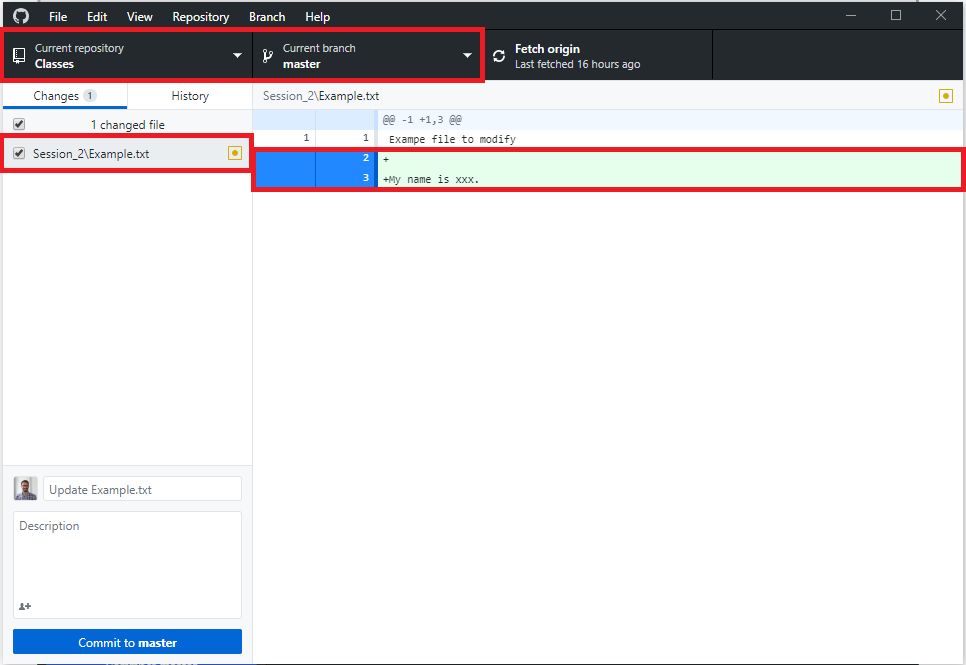
\includegraphics[width=0.7\linewidth]{../images/step2.A}
	\end{figure}
\end{frame}








\end{document}
